\documentclass[journal]{IEEEtran}

\usepackage{amsmath,amssymb,amsfonts}
\usepackage{booktabs}
\usepackage{cite}
\usepackage{graphicx}
\usepackage{float}
\usepackage{multirow}
\usepackage{placeins}
\usepackage{textcomp}
\usepackage{xcolor}
\usepackage{xspace}
\usepackage{url}

\graphicspath{{figures/}}
\DeclareGraphicsExtensions{.pdf,.png,.jpg}

\newcommand{\model}{CausalStreamingPPicker\xspace}
\newcommand{\modelv}{CausalStreamingPPicker\xspace}
\newcommand{\chunk}{0.5\,s\xspace}
\newcommand{\sr}{100\,Hz\xspace}
\newcommand{\spc}{50}
\newcommand{\RMS}{\mathrm{RMS}}
\newcommand{\tgrstablesetup}{\small\setlength{\tabcolsep}{2.6pt}\renewcommand{\arraystretch}{1.08}}
\newcommand{\tgrsdensetablesetup}{\footnotesize\setlength{\tabcolsep}{2.0pt}\renewcommand{\arraystretch}{1.06}}
\setlength{\textfloatsep}{6pt plus 1pt minus 2pt}
\setlength{\floatsep}{5pt plus 1pt minus 2pt}
\setlength{\intextsep}{6pt plus 1pt minus 2pt}
\setlength{\dbltextfloatsep}{6pt plus 1pt minus 2pt}
\setlength{\dblfloatsep}{5pt plus 1pt minus 2pt}
\setlength{\abovecaptionskip}{3pt}
\setlength{\belowcaptionskip}{0pt}

\begin{document}

\title{\model: Packet-Level Causal P-Wave Candidate Triggering in Strong-Motion Sensor Streams}

\author{Haoyu~Zhou and Qiang~Ma%
\thanks{Haoyu Zhou and Qiang Ma are with the Institute of Engineering Mechanics, China Earthquake Administration, No. 29 Xuefu Road, Harbin, Heilongjiang 150080, China (e-mail: zhouhaoyiu@gmail.com; maqiang@iem.ac.cn).}
\thanks{Corresponding author: Qiang Ma. Haoyu Zhou ORCID: 0009-0003-8817-1209.}
}

\markboth{IEEE Transactions on Geoscience and Remote Sensing}%
{Zhou: Causal P-Wave Candidate Triggering in Strong-Motion Streams}

\maketitle

\begin{abstract}
Strong-motion sensor networks acquire continuous acceleration streams for earthquake early warning, rapid ground-motion assessment, and engineering monitoring. The first geophysical information product in this stream is often a station-side P-wave candidate, which must be available within the near-source time budget before association, source-estimation, and ground-motion modules can operate. This article formulates that front-end task as packet-level causal processing and presents \modelv, a compact CNN--GRU picker for three-component strong-motion streams. Each \chunk, \sr packet is normalized with cumulative RMS statistics, augmented by a Z/NE particle-motion cue, encoded with left-padded causal convolutions, combined with inter-packet delta features, and passed to a unidirectional recurrent state. The design follows the physical transition from pre-event background to P-wave onset and keeps normalization, convolution, and trigger decisions chronological. The model has 275,827 parameters (1.08 MB) and needs 0.32 ms per packet in a single-thread CPU online benchmark. In a 1000-trace First-P replay, it obtains 98.9\% detection, median packet-index delay of 0.00 s, and 81.8\% of traces within $\pm$0.5 s. After InstanceGM pretraining and K-NET strong-motion adaptation, it reaches 100.0\% detection and 98.3\% usable picks on held-out K-NET strong-motion records, and 95.1\% detection with 80.6\% usable picks on the unseen Iquique benchmark. External labeled-accelerometer and continuous-stream audits further evaluate response near labeled P arrivals, low-SNR sensitivity, and station-day false triggers. The resulting stream is station-front-end P-candidate information for later association and source-estimation modules, and network-level logic issues alerts.
\end{abstract}

\begin{IEEEkeywords}
Earthquake early warning, P-wave candidate triggering, causal convolution, streaming inference, recurrent neural network, strong-motion acceleration sensors, geophysical signal processing.
\end{IEEEkeywords}

\section{Introduction}
\IEEEPARstart{S}{trong-motion} acceleration networks are geophysical sensor networks that convert ground motion into chronological data streams. For earthquake early warning (EEW), rapid ground-motion assessment, and engineering monitoring, the first useful data product is often a station-side P-wave candidate for association and source-estimation modules. Near-source stations leave little P--S separation for computation and communication. More distant stations give extra propagation time, yet attenuation, path effects, site response, and cultural noise can weaken the initial P signature. The central question is the data-arrival time at which a credible candidate first appears.

Operational front ends sit at the acquisition-and-processing boundary. Acceleration packets arrive in chronological order, station state is updated with small memory, and the output is a probability, time index, and confidence trail for downstream modules. Dense strong-motion and low-cost MEMS networks make this edge role important because station coverage controls warning opportunity and field links can degrade during damaging events \cite{chandrakumar2022memsreview,hu2021mems,wu2021palertreview}. Magnitude estimation, source location, and alert issuance remain downstream tasks.

This front-end role is also tied to a concrete strong-motion EEW workflow. Previous studies from the Institute of Engineering Mechanics and collaborators have developed P-arrival picking, EDP-Picker, on-site PGV/PGA prediction, and instrumental-intensity threshold models for early warning \cite{ma2013parrival,lu2020edppicker,song2021lssvmpgv,zhu2022hybridpgv,wang2023lstmtpga,li2024lstmintensity,li2024xgboostintensity}. Those downstream tasks need a timely and stable station-side P candidate before ground-motion prediction and network association can proceed. The workflow also separates earliest weak-P evidence, which controls warning time, from later amplitude and period growth, which is closer to PGV/PGA and instrumental-intensity products.

Classical STA/LTA and Baer--Kradolfer pickers are causal and simple, with known sensitivity to low SNR, nonstationary noise, and site-dependent thresholds \cite{allen1978automatic,baer1987automatic}. EDP-Picker is especially relevant because it combines P-wave energy and predominant-period information for early-warning onset picking \cite{lu2020edppicker}. Deep-learning pickers such as PhaseNet, EQTransformer, GPD, RED-PAN, AEnet, CapsPhase, SeisT, transfer-learning models, and unsupervised EQAnomalyNet have improved waveform representation, regional transfer, continuous detection, and annotation efficiency \cite{zhu2019phasenet,mousavi2020earthquake,ross2018gpd,liao2022redpan,guo2021aenet,saad2022capsphase,saad2024transfer,seist2024,wang2026eqanomalynet}. RED-PAN is the closest released real-time neural baseline because it adapts a 60 s multitask attention model to continuous phase picking through goal-oriented augmentation and output stabilization \cite{liao2022redpan}. These methods show the value of learned waveform features. The station-front-end question addressed here is when a usable candidate becomes available on the data-arrival time line.

Training and evaluation must follow the same packet clock. Many public PhaseNet- and EQTransformer-style interfaces are released and evaluated through completed waveform windows, and their offline metric is the pick or probability peak obtained after that window is available. The station protocol in this study is a packet sequence: each continuous record is divided into \chunk packets, packet labels are assigned around the labeled P arrival, and the loss is accumulated along the chronological sequence while the recurrent state advances. The test replay uses the same packet clock. PhaseNet and EQTransformer are evaluated as public fixed-window interfaces under causal replay, and RED-PAN is treated as the closest released continuous neural baseline.

Streaming use also changes preprocessing. Complete-window normalization can reach beyond packet time. Per-packet normalization is chronological and can suppress the amplitude growth that distinguishes an emergent P arrival from pre-event background. A low-latency neural picker needs chronology-preserving normalization, causal packet encoding, recurrent state update, and a trigger rule that can be audited at packet close.

This article presents \modelv, a compact CNN--GRU picker for packet-level strong-motion P-candidate generation. Each \chunk packet is normalized with cumulative RMS statistics, augmented with a Z/NE particle-motion cue, encoded by causal convolutions, combined with inter-packet delta features, and passed to a unidirectional GRU. The design ties the model to three seismological cues that matter in a station record: vertical-horizontal motion contrast, the local noise scale before P onset, and short-term energy growth as the P wave arrives.

The experiments use distinct data roles. InstanceGM supplies large mixed-sensor pretraining and component ablation data. K-NET provides the current public acceleration-network validation, with magnitude and distance bins, pre-P false-trigger replay, and event-window station association. Iquique tests unseen regional transfer. PNWAccelerometers provides an external labeled accelerometer response check with SNR-stratified results near labeled P arrivals. An independent public CI/FDSN continuous strong-motion campaign is used only for station-day false-trigger accounting. These public datasets test the station-front-end hypothesis under reproducible conditions; broader application can be evaluated with additional external strong-motion acceleration networks that provide verified P references. The main contributions are:
\begin{itemize}
  \item a packet-level causal formulation of station-side P-candidate triggering for strong-motion acceleration sensor streams;
  \item a lightweight CNN--GRU architecture that combines cumulative RMS normalization, Z/NE polarization, and embedding-space delta features;
  \item a held-out K-NET evaluation chain with external labeled-P and continuous-stream checks, reporting First-P timing, RED-PAN/PhaseNet/EQTransformer replay comparisons, magnitude and distance behavior, false-trigger control, and station-level association behavior.
\end{itemize}

Fig.~\ref{fig:task-positioning} summarizes the operating-time-line distinction that the rest of the paper evaluates.

\begin{figure*}[!t]
  \centering
  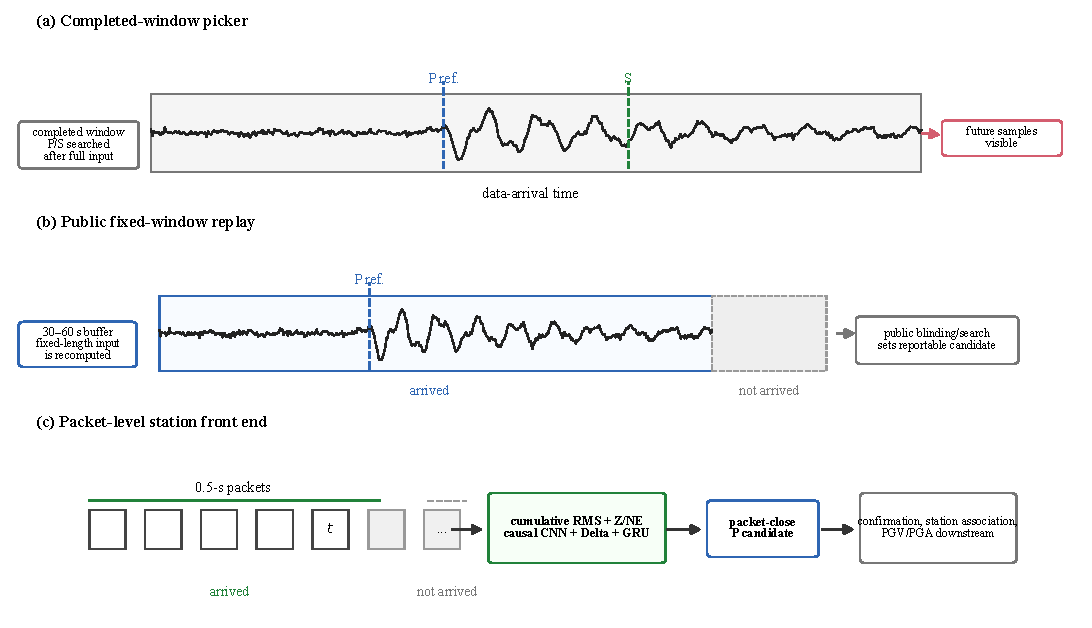
\includegraphics[width=\textwidth]{fig_task_positioning_en}
  \caption{Operational time lines for the station-front-end task. A completed-window picker can search P/S peaks after the event window is available. A public fixed-window interface can be replayed causally by feeding a trailing history buffer at each packet close, but its native blinding, search region, and window length still determine when a reportable candidate can appear. The proposed front end updates once per \chunk packet, carries causal state, emits a packet-close P candidate, and leaves confirmation, station association, and ground-motion products to downstream modules.}
  \label{fig:task-positioning}
\end{figure*}

\section{Related Work and Positioning}

Machine-learning phase pickers have matured around accurate P/S arrival estimation from labeled seismic waveforms, and unsupervised reconstruction methods such as EQAnomalyNet reduce pick-label dependence through anomaly scoring \cite{zhu2019phasenet,mousavi2020earthquake,ross2018gpd,perol2018cnn,pardo2019convpicking,mousavi2019cred,soto2021deepphasepick,zhou2019wenchuan,wang2026eqanomalynet}. EEW-oriented models add real-time constraints, compact inference, and continuous detection goals \cite{munchmeyer2020team,liao2022redpan,khan2022pdetector,ravishan2026lightweight,dtpp2026,tang2026seismodual,wibowo2024indonesia}. Strong-motion EEW studies further connect the P-wave front end to on-site PGV/PGA and instrumental-intensity prediction \cite{song2021lssvmpgv,zhu2022hybridpgv,wang2023lstmtpga,li2024lstmintensity,li2024xgboostintensity}. The present work uses these advances as baselines and design context, then narrows the evaluation to first candidate availability under chronological replay. This distinction matters because a complete-record anomaly peak, an offline probability peak, and an online first trigger answer different operational questions.

The data setting is also specific. INSTANCE/InstanceGM, K-NET-derived labeled records, Iquique, and other standardized SeisBench datasets enable reproducible training and transfer tests \cite{michelini2021instance,aoi2004knet,nied2019knet,sarkar2022japan,magrini2020dataset,woollam2019iquique,woollam2022seisbench}. K-NET is central here because it is a dense strong-motion accelerometer network and matches the target station-front-end use case. InstanceGM is used for representation learning across seismic velocity and strong-motion acceleration channels; the final strong-motion timing claim is anchored by the held-out K-NET accelerometer test.

\section{Method}

\subsection{Operational Design Target}
The design target is the waveform-to-candidate stage of an edge--cloud geophysical sensing chain for EEW and rapid engineering response. The station front end receives a continuous acceleration stream, emits a candidate P trigger and probability, and passes that candidate to later association, location, magnitude-estimation, and alert-decision modules. This stage matches the point at which strong-motion stations and dense MEMS nodes first convert waveform samples into information that can be used by an engineering monitoring system.

Three geophysical and engineering constraints drive the model. First, near-source records leave little P--S separation for computation, communication, and association, so the first useful output must occur within one or a few packet intervals after the P onset. Second, records at larger distance still matter for network corroboration, yet their first arrivals may have lower SNR and stronger path or site variability. Third, a single-station P candidate is front-end evidence for a downstream network decision. The model must keep the early candidate available, while confirmation length, false-trigger replay, and multi-station coincidence control how that candidate is used. These constraints explain why the method emphasizes causal normalization, packet-to-packet change, distance-binned K-NET testing, pseudo-continuous pre-P noise replay, and event-window association.

\subsection{Problem Formulation}
Let $\mathbf{x}_t \in \mathbb{R}^{3\times L}$ be the $t$-th three-component waveform packet, where $L=\spc$ samples at \sr, corresponding to \chunk. Given packets $\mathbf{x}_{1:t}$, the picker emits a scalar probability $p_t \in [0,1]$ that the P arrival has occurred in or near packet $t$. Packet-level causality requires
\begin{equation}
  p_t = f(\mathbf{x}_1,\ldots,\mathbf{x}_t), \qquad
  p_t \not\equiv f(\mathbf{x}_{t+1},\ldots).
\end{equation}
In streaming inference, hidden states are carried forward and no earlier packet is reprocessed.

The complete packet-level data path is summarized in Fig.~\ref{fig:architecture}. The following subsections describe the online normalization, packet encoder, delta construction, recurrent state update, and trigger rule.

\begin{figure*}[!t]
  \centering
  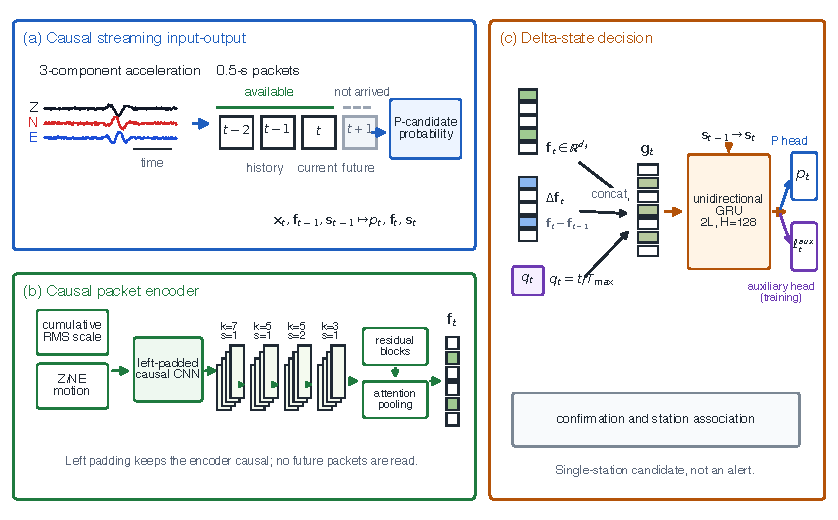
\includegraphics[width=\textwidth]{fig_architecture_en}
  \caption{Delta-enhanced streaming architecture of \modelv for station-side P-wave candidate triggering. Panel (a) shows the causal packet-level input-output path from three-component waveforms to packet-close P-candidate probability. Panel (b) expands the causal CNN encoder with cumulative RMS scaling, the Z/NE polarization feature, left-padded convolutions, residual blocks, and temporal attention pooling. Panel (c) shows how the encoder output, inter-packet Delta feature, and relative position enter the unidirectional GRU, and marks confirmation and station association as downstream steps.}
  \label{fig:architecture}
\end{figure*}

\subsection{Causal Packet Normalization}
\label{sec:norm}
For each packet, the channel-wise DC offset is removed using only samples inside that packet. Let $\mathbf{u}_t$ be the centered packet and $n_t$ the number of valid samples, excluding zero padding in the final packet. The packet energy is
\begin{equation}
  e_t = \frac{1}{3 n_t}\sum_{c=1}^{3}\sum_{i=1}^{n_t} u_{t,c,i}^2 .
\end{equation}
The running mean square $m_t$ is updated by a weighted online mean-square rule,
\begin{equation}
  c_t = c_{t-1}+n_t,\qquad
  m_t = m_{t-1} + \frac{n_t}{c_t}(e_t-m_{t-1}),
\end{equation}
with $m_0=0$ and $c_0=0$. The normalized packet is
\begin{equation}
  \tilde{\mathbf{x}}_t = \frac{\mathbf{u}_t}{\sqrt{m_t}+\epsilon}.
\end{equation}
This cumulative RMS rule is causal and preserves the relative amplitude increase at P onset because the denominator evolves smoothly with the accumulated trace history. Complete-window z-score normalization uses future samples in an online setting. Per-packet z-score normalization can suppress onset amplitude. The input-level rule used here preserves packet-order causality and onset-related amplitude growth in a streaming trace, complementing neural normalization layers used inside deep networks \cite{ioffe2015batchnorm,ba2016layernorm,wu2018groupnorm,zhang2019rmsnorm}.

\subsection{Polarization Channel}
The model uses a lightweight physically motivated polarization proxy computed sample-wise from the normalized Z, N, and E channels:
\begin{equation}
  r_{t,i} = \log\left(1 + \frac{\tilde{x}_{t,Z,i}^{2}}
  {\tilde{x}_{t,N,i}^{2}+\tilde{x}_{t,E,i}^{2}+\epsilon}\right).
\end{equation}
The ratio approximates the relative vertical-to-horizontal energy concentration and gives the CNN explicit access to a P-wave-relevant particle-motion cue, following the broader use of three-component polarization analysis in seismology \cite{jurkevics1988polarization}. This channel is intentionally simple. Incidence angle, back azimuth, rectilinearity, and full covariance-based polarization state are outside its scope. Strong near-source shaking, site response, instrument orientation errors, and regional propagation can all weaken a ratio-based rule. The trigger uses $r_{t,i}$ together with the normalized Z, N, and E channels and with GRU delta features that summarize how the learned packet representation changes relative to the immediate background. The resulting CNN input is $\mathbf{z}_t \in \mathbb{R}^{4\times L}$.

\subsection{Causal CNN Packet Encoder}
The packet encoder contains four left-padded one-dimensional convolutional layers followed by two residual causal blocks and attention pooling. Every convolution uses padding only on the left, so the feature at sample $i$ can depend only on samples $1,\ldots,i$. The channel schedule is $4\rightarrow16\rightarrow32\rightarrow64\rightarrow64$, with kernel sizes $7,5,5,3$ and a stride-2 downsampling at the third convolution. Each residual block follows the residual-learning principle of ResNet while preserving causal padding \cite{he2016resnet}. Temporal attention pooling maps the final feature map to a packet embedding $\mathbf{f}_t\in\mathbb{R}^{64}$:
\begin{equation}
  \mathbf{f}_t = \sum_i \alpha_{t,i}\mathbf{h}_{t,i},\qquad
  \alpha_{t,i} = \mathrm{softmax}_i(g(\mathbf{h}_{t,i})).
\end{equation}

\subsection{Delta Features, Position Encoding, and GRU State}
Because P arrivals are characterized by changes in waveform statistics, the model passes both the packet embedding and its first difference to the recurrent layer:
\begin{equation}
  \Delta \mathbf{f}_t =
  \begin{cases}
    \mathbf{0}, & t=1,\\
    (\mathbf{f}_t-\mathbf{f}_{t-1})/\sqrt{2}, & t>1.
  \end{cases}
\end{equation}
The division by $\sqrt{2}$ keeps the delta feature scale comparable to the embedding scale under an independent equal-variance approximation. A normalized scalar position $q_t=t/T_{\max}$, with $T_{\max}=320$, is appended to the recurrent input:
\begin{equation}
  \mathbf{g}_t = [\mathbf{f}_t;\Delta\mathbf{f}_t;q_t]\in\mathbb{R}^{129}.
\end{equation}
A two-layer unidirectional GRU with hidden size 128 updates the state \cite{cho2014gru}
\begin{equation}
  \mathbf{s}_t = \mathrm{GRU}(\mathbf{g}_t,\mathbf{s}_{t-1}),
\end{equation}
and two linear heads produce the P-arrival logit $\ell_t$ and an auxiliary logit used in component studies. The P probability is $p_t=\sigma(\ell_t)$.

The delta path is the main mechanism that turns the model from a static packet classifier into an onset detector. A local P arrival changes short-window waveform shape, frequency content, and energy relative to the packets immediately before it. Near-source traces may show a sharp increase within one packet; more distant or noisy traces may show a weaker multi-packet rise. By feeding $\mathbf{f}_t$ and $\Delta\mathbf{f}_t$ together, the GRU can use both the current particle-motion pattern and the direction of recent change.

\subsection{Training Objective and Detection Rule}
Training uses Gaussian-smoothed packet labels centered at the labeled P-arrival packet. Let $y_t\in[0,1]$ be the target label and $M_t$ a validity mask. The reported multi-domain checkpoint is optimized with a masked binary cross-entropy detection loss:
\begin{equation}
  \mathcal{L}_{p}=
  \frac{\sum_t M_t\,\mathrm{BCE}(\ell_t,y_t)}{\sum_t M_t}.
\end{equation}
Auxiliary-head supervision and pre-P probability shaping are evaluated in the component ablation configuration, while the inference rule remains unchanged across variants. At inference time, the first-trigger decision is the earliest packet whose probability reaches the decision threshold $\theta$. The First-P replay uses $\theta=0.30$ for \modelv{} as a permissive candidate-generation operating point, $\theta=0.50$ for PhaseNet, and $\theta_P=0.10$ for EQTransformer; the multi-domain and ablation summaries use $\theta=0.55$ unless a different operating point is stated. For confirmation analysis, a trigger becomes available after $k$ consecutive packets exceed $\theta$, and its delay is measured at the close of the $k$-th packet. Candidate triggers are station-level evidence; early-trigger risk is evaluated separately and reduced by confirmation or station association. Thresholds are selected on the development split and fixed for the reported test sets.

\section{Experimental Setup}

\subsection{Data Roles and Splits}
The experiments are organized around distinct evidence roles. InstanceGM supplies broad pretraining and component-ablation data. Local metadata contain 1,159,249 traces from 54,008 events and include both seismic velocity records and strong-motion acceleration records; for $M\geq4$, the subset contains 15,038 seismic-velocity traces and 5,378 strong-motion acceleration traces. K-NET is the target public strong-motion validation set because it gives accelerometer records from a dense operational network. The local K-NET metadata contain 21,141 accelerometer traces from 1,528 event groups, including 15,473 $M\geq4$ traces from 845 event groups. Iquique is a third-domain transfer test and is kept out of training and model selection. PNWAccelerometers is used as an external labeled accelerometer check of response near labeled P arrivals; continuous-stream first-trigger behavior is evaluated in the false-trigger audits.

\begin{table*}[!t]
\centering
\caption{Dataset scale, evidence roles, and scope. Counts describe the local metadata used by this study; public waveform redistribution follows the original data-provider licenses.}
\label{tab:dataset_roles}
{\tgrsdensetablesetup
\begin{tabular}{@{}p{0.15\textwidth}p{0.21\textwidth}p{0.18\textwidth}p{0.21\textwidth}p{0.18\textwidth}@{}}
\toprule
Dataset & Local scale & Record type & Evidence role & Scope\\
\midrule
InstanceGM & 1,159,249 traces from 54,008 events; $M\geq4$ subset includes 15,038 velocity and 5,378 acceleration traces & mixed seismic velocity and strong-motion acceleration records & representation learning, component ablation, and sensor-family stress testing & pretraining and mechanism analysis; strong-motion claims are anchored by acceleration tests\\
K-NET & 21,141 accelerometer traces from 1,528 event groups; held-out test uses 715 $M\geq4$, distance $\leq$200 km traces & dense Japanese strong-motion accelerometer network & target public strong-motion validation with timing, RED-PAN comparison, false-trigger replay, and station association & public acceleration validation within the tested magnitude-distance range\\
Iquique & 4001 valid P-labeled traces in the blind-domain evaluation & regional seismic benchmark outside the training mixture & unseen-region transfer check & cross-region transfer evidence, excluded from model selection\\
PNWAccelerometers & 500 high-SNR labeled records plus 500 unfiltered random records in the external check & public accelerometer records with labeled P arrivals & external response near labeled P arrivals and SNR-stratified quality check & response near labeled P arrivals check; continuous-stream behavior is evaluated separately\\
\bottomrule
\end{tabular}}
\end{table*}

The K-NET split is event-level: records from the same catalog event group do not cross training, development, and test subsets. The reported K-NET test result uses held-out $M\geq4.0$ records with epicentral distance $\leq200$ km, yielding 715 traces. K-NET magnitude and distance bins are reported to connect the result to near-source and intermediate-distance station needs. The Iquique test uses 4001 valid P-labeled traces from northern Chile \cite{woollam2019iquique,woollam2022seisbench}. PNWAccelerometers is accessed through SeisBench and evaluated with the frozen checkpoint in a search beginning three packets before the labeled P-arrival packet \cite{woollam2022seisbench}. Public waveform data are obtained through their original providers or SeisBench, and raw third-party waveforms are not redistributed \cite{michelini2021instance,aoi2004knet,nied2019knet,sarkar2022japan}.

\subsection{Baselines and Replay Protocol}
PhaseNet, EQTransformer, RED-PAN, and recursive STA/LTA are compared under chronological replay \cite{zhu2019phasenet,mousavi2020earthquake,liao2022redpan,woollam2022seisbench}. The comparison uses released public interfaces and weights where available, and evaluates first candidate availability on the station time line. Offline accuracy after retraining or task-specific redesign is outside this protocol. \modelv{} receives each \chunk packet once, carries its recurrent state forward, and emits $p_t$ at packet close. PhaseNet and EQTransformer use their public fixed-window interfaces: at each packet close, they receive a native-length trailing window ending at the current time, with zero fill only before the event record begins. EQTransformer keeps the public 5 s blinding and the P threshold of 0.1. RED-PAN is replayed on the common K-NET $M\geq4$ records with its released 60 s model; each window uses only samples available up to packet close.

The main timing metric is First-P delay, measured between the first trigger packet and the labeled P-arrival packet. Negative values indicate early triggers. Perfect picks fall within $\pm1$ packet, and usable picks fall within $\pm3$ packets unless another tolerance is stated. Because \modelv{} emits at packet close, sample-level availability can differ from packet-index delay by up to one \chunk packet. Pseudo-continuous false-trigger replay concatenates held-out K-NET pre-P fragments by station, carries station state within each stream, and excludes two packets after each fragment boundary to avoid artificial concatenation effects.

\subsection{Training and Implementation}
The model is implemented in PyTorch with encoder hidden size 64, GRU hidden size 128, two GRU layers, dropout 0.15--0.25, and $T_{\max}=320$. Training uses AdamW \cite{loshchilov2019adamw}, Gaussian packet labels with $\sigma=1.5$, batch size 4 with 8-step gradient accumulation, and a maximum sequence length of 320 packets. Each trace is presented as an arrival-ordered packet sequence. The target label at every packet is computed from the labeled P-arrival packet, and gradients are accumulated over valid packet positions, matching the causal replay protocol. Training follows two stages: InstanceGM pretraining, then mixed InstanceGM/K-NET training for strong-motion adaptation. K-NET training and development records are used only in the second stage; the reported K-NET metrics use the held-out event-level test subset.

\section{Results}

\subsection{Computational Efficiency}
Table~\ref{tab:efficiency} summarizes model size, recomputed waveform samples per decision update, and measured forward latency. \modelv{} processes only the new \chunk packet and carries a GRU state. Fixed-window models reprocess a 30--60 s waveform window for each native call or sliding update.

\begin{table}[!t]
\centering
\caption{Deployment-oriented complexity and latency. Samples/update counts waveform samples reprocessed at each decision update. Forward time reports mean/P95 in milliseconds. The proposed-row latency is a single-thread CPU online packet-step measurement including cumulative RMS normalization, tensor conversion, model forward pass, sigmoid, and recurrent-state update, excluding disk I/O.}
\label{tab:efficiency}
{\tgrsdensetablesetup
\begin{tabular}{@{}lccccc@{}}
\toprule
Model & Params & Size & Samples & Input & Fwd.\\
\midrule
Proposed & 275,827 & 1.08 MB & 50 & pkt. & 0.32/0.34\\
PhaseNet & 268,443 & 1.06 MB & 3001 & 30 s & 3.94/4.83\\
EQTrans. & 376,935 & 1.44 MB & 6000 & 60 s & 20.79/25.42\\
RED-PAN & 352,817 & 1.35 MB & 6000 & 60 s & 114.24/123.12\\
\bottomrule
\end{tabular}}
\end{table}

The single-thread CPU benchmark gives 0.31 ms median and 0.34 ms P95 packet-step latency for \modelv{}. Replaying a 30 s trace with 60 packet updates takes 18.84 ms on average, less than 0.1\% of the physical packet interval. This separates compute time from warning latency: a short forward pass after a long input window is still unavailable until the window has arrived.

\subsection{First-P Latency}
Table~\ref{tab:firstp} and Fig.~\ref{fig:firstp} give the First-P delay statistics over 1000 streaming-replayed traces: 500 InstanceGM test traces and 500 held-out K-NET test traces sampled under the same magnitude filter and replay grid. At the permissive candidate threshold, \modelv{} detects 98.9\% of traces, has a median packet-index delay of 0.00 s relative to the labeled P-arrival packet, and places 81.8\% of all traces within $\pm$0.5 s. With causal left-prefilled native windows, PhaseNet detects 99.9\% of traces but shifts strongly to pre-P triggers, with a median delay of -13.50 s and 5.9\% within $\pm$0.5 s. EQTransformer detects 99.9\% of traces under the same prefilled protocol and remains late, with a +20.00 s median delay and 0.2\% within $\pm$0.5 s. These values characterize packet-index candidate timing under the reset event-window replay. Sample-level availability and continuous-stream false-trigger behavior are evaluated separately below.

\begin{table*}[!t]
\centering
\caption{First-P detection delay summary over 1000 traces. Delay is measured by packet index relative to the labeled P-arrival packet; packet-close availability can add up to one \chunk packet within a detected packet. PhaseNet and EQTransformer use causal left-prefilled native windows, with no future samples.}
\label{tab:firstp}
{\tgrsdensetablesetup
\begin{tabular}{@{}p{0.14\textwidth}p{0.19\textwidth}p{0.16\textwidth}cccccc@{}}
\toprule
Model & Causal replay input & Candidate rule & Det. & Mean & Med. & P95 & $\pm$0.5 s & $\pm$1.0 s\\
\midrule
Proposed & one \chunk packet plus carried GRU state & first $p_t\geq0.30$ & 98.9\% & -0.38 s & 0.00 s & +0.50 s & 81.8\% & 89.7\%\\
PhaseNet (prefill) & 30 s native trailing window, causal left fill & first $p_t\geq0.50$ & 99.9\% & -11.34 s & -13.50 s & +0.50 s & 5.9\% & 7.7\%\\
EQTrans. (prefill) & 60 s native trailing window plus public 5 s blinding & first $p_t^P\geq0.10$ & 99.9\% & +20.90 s & +20.00 s & +37.00 s & 0.2\% & 0.3\%\\
STA/LTA & recursive causal characteristic function & threshold 4.0 & 79.7\% & +6.36 s & +1.50 s & +27.00 s & 20.1\% & 32.7\%\\
\bottomrule
\end{tabular}}
\end{table*}

\begin{figure}[!t]
  \centering
  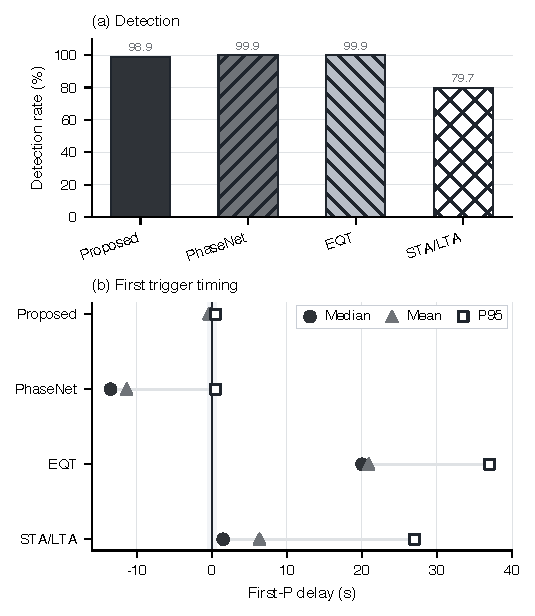
\includegraphics[width=\columnwidth]{fig1_firstp_latency_en_column}
  \caption{First-P streaming latency comparison for \modelv, PhaseNet, EQTransformer, and STA/LTA. The public window pickers are replayed with history-buffer-aligned native windows, so the comparison reflects first-trigger behavior under their public fixed-window interfaces.}
  \label{fig:firstp}
\end{figure}

The methods exhibit different first-trigger error modes under the same chronological replay protocol. \modelv{} is concentrated around zero delay, with early outliers consistent with pre-P noise growth or packet-boundary quantization. STA/LTA has a long positive tail because weak signals often require additional amplitude accumulation before the trigger condition is met. Under history-buffer-aligned native-window replay, the public PhaseNet threshold often converts pre-P probability growth inside the event window into an early trigger. EQTransformer keeps its 60 s native input, 5 s blinding, and public P-pick threshold, and its reportable P pick remains late in this replay. These results show that online First-P behavior depends on window organization, blinding, thresholds, search regions, and single-window forward time as distinct factors.

A threshold and right-edge search sweep was added for public window pickers. PhaseNet reaches at most 20.5\% within $\pm$0.5 s under a last-1 s search, with 90.0\% detection and a -6.50 s median delay; among settings with at least 95\% detection, the best $\pm$0.5 s rate is 17.3\%. EQTransformer reaches at most 1.3\% within $\pm$0.5 s under the tested public-window settings. These sweeps leave the same conclusion: fixed-window public interfaces and First-P station-front-end timing answer different timing questions.

Fig.~\ref{fig:causal-replay-case} gives a representative K-NET replay and exposes the packet-level cues behind one confirmed candidate.

\begin{figure*}[!t]
  \centering
  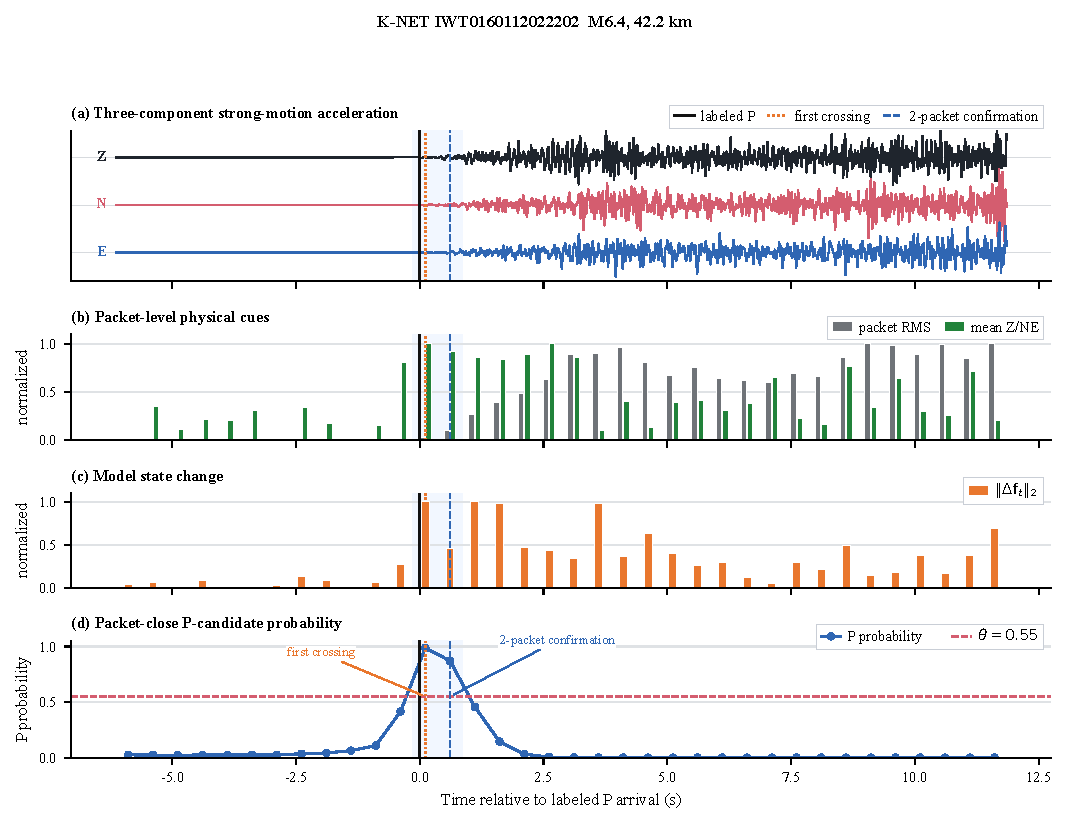
\includegraphics[width=\textwidth]{fig_causal_replay_case_en}
  \caption{Packet-level causal replay on a held-out K-NET strong-motion record (IWT0160112022202, M6.4, epicentral distance 42.2 km). The vertical black line marks the labeled P arrival. The gray and green bars show chronological packet RMS and mean Z/NE cues after causal normalization; the orange bars show the norm of the embedding-space Delta feature used by the GRU. The bottom panel shows packet-close P-candidate probability, the $\theta=0.55$ threshold, the first threshold crossing, and the two-packet confirmation time. This case illustrates the per-packet decision path; aggregate timing, false-trigger, and association results are reported in the tables.}
  \label{fig:causal-replay-case}
\end{figure*}

\subsection{Multi-Domain and Blind-Domain Performance}
Tables~\ref{tab:domains} and \ref{tab:station_detailed} give the multi-domain and blind-domain results. After InstanceGM pretraining and mixed InstanceGM/K-NET training, the model obtains 100.0\% detection, 98.3\% usable picks, and 92.9\% perfect picks on the filtered K-NET strong-motion test set. On Iquique, which is not part of the training mixture, the model maintains 95.1\% detection and 80.6\% usable picks under unseen regional conditions. The detailed table separates the mixed InstanceGM sensor families and shows that strong-motion acceleration traces are harder than seismic velocity traces under the same checkpoint, supporting the need for explicit strong-motion validation.

\begin{table}[!t]
\centering
\caption{Multi-domain and blind-domain evaluation. The InstanceGM subset contains 2000 traces for ablation, the InstanceGM summary contains 5705 validation traces, and timing offset is in \chunk packets.}
\label{tab:domains}
{\tgrstablesetup
\begin{tabular}{@{}lccccc@{}}
\toprule
Domain & $n$ & Det. & Usable & Perfect & Mean offset\\
\midrule
InstanceGM subset & 2000 & 85.05\% & 82.75\% & 73.35\% & +0.78\\
InstanceGM summary & 5705 & 99.5\% & 88.9\% & 72.3\% & +0.3\\
K-NET test & 715 & 100.0\% & 98.3\% & 92.9\% & -0.87\\
Iquique test & 4001 & 95.1\% & 80.6\% & 74.5\% & -1.71\\
\bottomrule
\end{tabular}}
\end{table}

\begin{table*}[!t]
\centering
\caption{Detailed station-level P-candidate results by data slice. Category counts are ordered as perfect/good/early/late/missed. MAE, RMSE, and timing offsets are detected-trace errors in seconds; Iquique is included as a summary-only blind-domain row because the current release keeps only aggregate category counts.}
\label{tab:station_detailed}
{\tgrsdensetablesetup
\begin{tabular}{@{}llrcccclccc@{}}
\toprule
Data slice & Group & $n$ & Det. & Usable & Perfect & Category counts & MAE & RMSE & Med. offset & $\sigma$\\
\midrule
InstanceGM $M\geq4$ & all & 2000 & 89.6\% & 85.7\% & 79.3\% & 1586/128/41/38/207 & 0.41 & 1.04 & 0.00 & 1.04\\
InstanceGM $M\geq4$ & seismic & 1507 & 91.5\% & 88.3\% & 82.5\% & 1243/88/25/23/128 & 0.36 & 0.81 & 0.00 & 0.80\\
InstanceGM $M\geq4$ & strong-motion & 493 & 84.0\% & 77.7\% & 69.6\% & 343/40/16/15/79 & 0.58 & 1.60 & 0.00 & 1.59\\
InstanceGM $M<4$ & all & 2000 & 79.0\% & 73.5\% & 68.3\% & 1366/103/47/65/419 & 0.58 & 1.99 & 0.00 & 1.99\\
InstanceGM $M<4$ & seismic & 1412 & 82.7\% & 78.0\% & 72.7\% & 1026/75/19/48/244 & 0.44 & 1.26 & 0.00 & 1.26\\
InstanceGM $M<4$ & strong-motion & 588 & 70.2\% & 62.6\% & 57.8\% & 340/28/28/17/175 & 0.97 & 3.28 & 0.00 & 3.24\\
K-NET $M\geq4$, $d\leq200$ km & all & 715 & 100.0\% & 98.3\% & 92.9\% & 664/39/12/0/0 & 0.43 & 1.15 & -0.50 & 1.07\\
K-NET $M<4$, $d\leq200$ km & all & 316 & 100.0\% & 99.4\% & 99.4\% & 314/0/2/0/0 & 0.20 & 0.56 & 0.00 & 0.52\\
Iquique blind region & all & 4001 & 95.1\% & 80.6\% & 74.5\% & 2979/247/575/3/197 & -- & -- & -- & --\\
\bottomrule
\end{tabular}}
\end{table*}


Table~\ref{tab:redpan_knet} adds the aligned K-NET picking comparison requested by the baseline hierarchy. The official RED-PAN 60 s model is the strongest directly executed real-time neural baseline for this table \cite{liao2022redpan}. On the same 715 records, RED-PAN reaches 98.6\% detection, 98.2\% usable picks, and 97.8\% perfect picks. \modelv{} gives a similar usable rate, 100.0\% detection, and no misses under the packet-level causal replay. The public EQTransformer model detects all 715 records in the causal trailing-window diagnostic, but its first online P candidate is usually late when the public 5 s window blinding is retained; the P-only replay gives 0.1\% usable picks and a median delay of +26 packets, and the detection-gated sensitivity check gives no usable picks. The comparison indicates that the proposed lightweight packet-state model is competitive with a strong real-time neural baseline on held-out K-NET strong-motion records and avoids the online-availability delay of public full-window pickers.

\begin{table*}[!t]
\centering
\caption{Detailed aligned K-NET comparison on the common 715 $M\geq4$ held-out strong-motion records. Category counts are ordered as perfect/good/early/late/missed using the $\pm$1-packet perfect and $\pm$3-packet usable definitions; timing offset is in \chunk packets. The EQTransformer row uses the public SeisBench \texttt{original} weights, P threshold 0.1, and 5 s left/right blinding.}
\label{tab:redpan_knet}
{\tgrsdensetablesetup
\begin{tabular}{@{}p{0.15\textwidth}p{0.21\textwidth}ccccccc@{}}
\toprule
Model & Online input contract & Det. & Usable & Perfect & Category counts & Mean offset & Med. offset & SD offset\\
\midrule
Proposed & one \chunk packet plus causal GRU state & 100.0\% & 98.3\% & 92.9\% & 664/39/12/0/0 & -0.87 & -1.0 & 2.13\\
RED-PAN 60s & 60 s trailing window, 0.5 s replay step & 98.6\% & 98.2\% & 97.8\% & 699/3/2/1/10 & +0.26 & 0.0 & 12.49\\
EQT original & 60 s trailing window with 5 s public blinding & 100.0\% & 0.1\% & 0.0\% & 0/1/1/713/0 & +28.73 & +26.0 & 14.62\\
\bottomrule
\end{tabular}}
\end{table*}

\begin{table*}[!t]
\centering
\caption{K-NET strong-motion stratified results for the held-out $M\geq4$, distance $\leq$200 km subset. Rows share the same $\theta=0.55$ one-packet candidate rule used in Table~\ref{tab:redpan_knet}.}
\label{tab:knet_stratified_detailed}
{\tgrsdensetablesetup
\begin{tabular}{@{}llrcccclccc@{}}
\toprule
Stratum & Type & $n$ & Det. & Usable & Perfect & Category counts & MAE & RMSE & Mean offset & Med. offset\\
\midrule
$M\geq4$, $d\leq200$ km & all & 715 & 100.0\% & 98.3\% & 92.9\% & 664/39/12/0/0 & 0.43 & 1.15 & -0.43 & -0.50\\
M4--5 & magnitude & 535 & 100.0\% & 99.1\% & 98.1\% & 525/5/5/0/0 & 0.33 & 0.79 & -0.33 & -0.50\\
M5--6 & magnitude & 105 & 100.0\% & 96.2\% & 89.5\% & 94/7/4/0/0 & 0.53 & 1.39 & -0.53 & -0.50\\
M6--7 & magnitude & 75 & 100.0\% & 96.0\% & 60.0\% & 45/27/3/0/0 & 1.07 & 2.33 & -1.07 & -0.50\\
0-50 km & distance & 306 & 100.0\% & 98.0\% & 93.8\% & 287/13/6/0/0 & 0.37 & 0.84 & -0.37 & -0.50\\
50-100 km & distance & 340 & 100.0\% & 98.5\% & 93.2\% & 317/18/5/0/0 & 0.47 & 1.31 & -0.47 & -0.50\\
100-200 km & distance & 69 & 100.0\% & 98.6\% & 87.0\% & 60/8/1/0/0 & 0.54 & 1.47 & -0.54 & -0.50\\
\bottomrule
\end{tabular}}
\end{table*}


Fig.~\ref{fig:knet} further breaks down the K-NET result by magnitude and distance. The result is dominated by near-packet picks: 664 of 715 traces are perfect, 39 are good, 12 are early, and none are missed. Magnitude-bin usable rates remain between 96.0\% and 99.1\% for M4--M7, while distance-bin usable rates are 98.0\%, 98.5\%, and 98.6\% for 0--50 km, 50--100 km, and 100--200 km, respectively. The lower perfect rate in the largest-magnitude bin suggests that strong local shaking complexity can affect packet-level timing even when detections remain usable.

\begin{figure*}[!t]
  \centering
  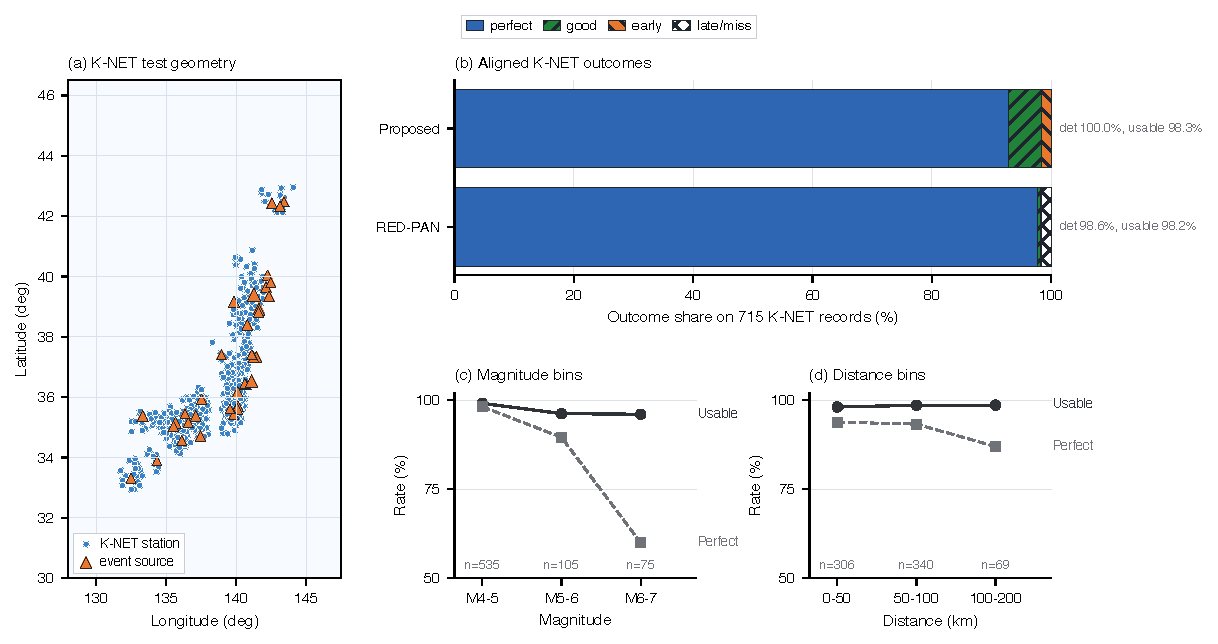
\includegraphics[width=\textwidth]{fig2_knet_bins_en_column}
  \caption{K-NET strong-motion evaluation summary for the common $M\geq4$ and distance $\leq$200 km held-out set. Panel (a) shows the test-record station and source geometry. Panel (b) compares outcome categories for \modelv{} and the released RED-PAN 60 s model on the same 715 records. Panels (c) and (d) show usable and perfect rates for \modelv{} across magnitude and distance bins.}
  \label{fig:knet}
\end{figure*}

The distance bins connect the experiment to the near- and intermediate-field requirement. The 0--50 km group is the most timing-sensitive part of the filtered K-NET set because little warning time remains after the first local P arrival. The 100--200 km group gives more propagation time but tests whether the candidate trigger remains stable when path effects and lower onset amplitude can make first arrivals less distinct. The similar usable rates across these bins indicate that the tested model did not trade near-source speed for a collapse at larger distances within this held-out subset. The conclusion is limited to the reported distance range and event-window replay.

The Iquique blind-domain result is more challenging. The model detects 95.1\% of traces, and the mean timing offset shifts to -1.71 packets, indicating a stronger tendency toward early triggers. This behavior is consistent with a domain shift in path effects, aftershock background, and station noise. For a new network, threshold calibration has to be paired with short-history probability-shape checks and multi-station consistency before public alerting.

Fig.~\ref{fig:knet-imperfect-association} visualizes representative non-perfect two-packet confirmation cases and the event-window association gate. The examples show an early confirmation, a usable but early confirmation, and a record without two-packet confirmation; the association panel shows how station candidates can still form a three-station timing window without revising the individual station triggers.

\begin{figure*}[!t]
  \centering
  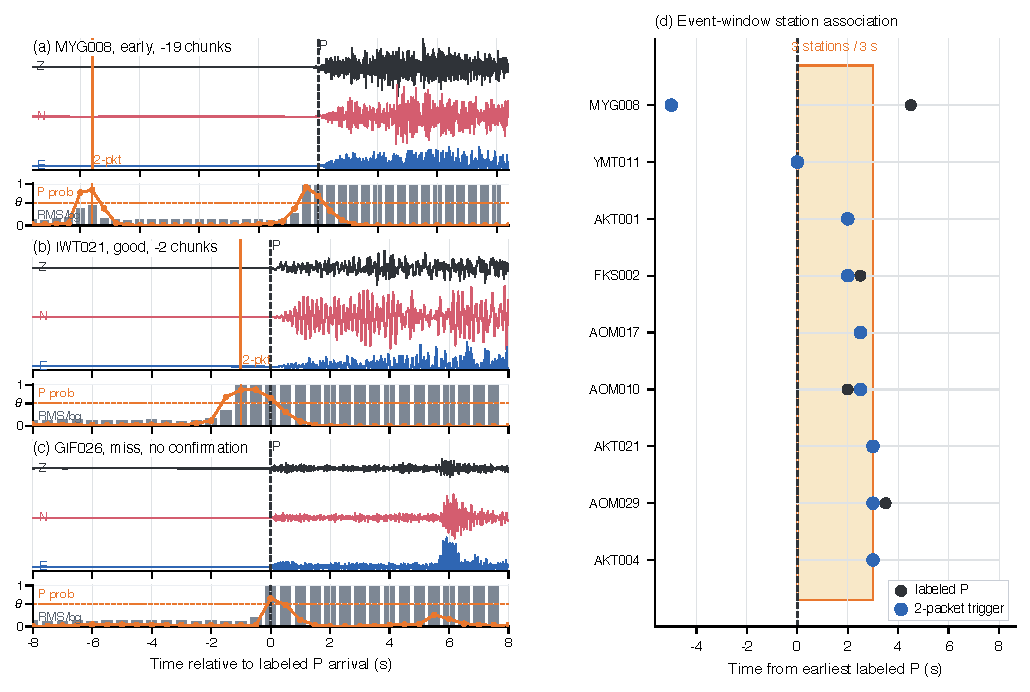
\includegraphics[width=\textwidth]{fig_knet_imperfect_association_en}
  \caption{Representative K-NET non-perfect two-packet confirmation cases and event-window association logic. Panels (a)--(c) show three-component strong-motion records relative to the labeled P arrival, with the orange line marking the two-packet confirmation time when it exists. The lower strip under each waveform overlays packet RMS relative to the pre-P median (gray bars, clipped at 6$\times$ and scaled to the strip height), packet-close P-candidate probability (orange curve), and the working threshold $\theta=0.55$ (orange dashed line). Panel (d) shows station trigger times for one event relative to the earliest labeled P arrival; the shaded band marks a three-station/3 s association window.}
  \label{fig:knet-imperfect-association}
\end{figure*}

The three lower probability/RMS strips separate distinct boundary mechanisms. MYG008 is an isolated early candidate. Its two-packet confirmation ends at chunk 9, whereas the labeled P arrival is at chunk 28, giving a -19 chunk (-9.5 s) availability gap. The gray RMS bars at the two confirming packets are only about 2.6$\times$ and 3.1$\times$ the pre-P background median, while the labeled-P and following packets reach roughly 163$\times$ and 285$\times$ the same background level. The orange probability curve is the decisive evidence: it crosses $\theta=0.55$ for two consecutive pre-P packets during a moderate local fluctuation, so the station can report an early candidate before the main P onset appears in the waveform. The event-window panel then places this station trigger 5.0 s before the earliest labeled P arrival and outside the first three-station/3 s association window. This is the type of single-station early response that network timing consistency is meant to contain.

IWT021 is a usable early case. The two-packet confirmation ends two chunks before the labeled P arrival, or 1.0 s early. Its RMS strip rises in the last seconds before the label: about 2.4$\times$, 6.4$\times$, and 22.8$\times$ the pre-P background in the three packets immediately preceding the labeled P packet. The probability curve rises with that ramp and remains above $\theta=0.55$ for the required two packets. The timing offset is negative, but the evidence follows the developing onset energy and differs from an isolated pre-P spike. This places the record inside the usable packet-level margin and outside the perfect packet-match category.

GIF026 gives the complementary failure mode. The waveform energy is clear at and after the label: the labeled-P packet and following packet are about 50.9$\times$ and 55.7$\times$ the pre-P background median. The orange probability curve still forms no two-packet run above $\theta=0.55$ at the working point. The miss comes from a short or unstable learned probability response under the two-packet confirmation rule; waveform energy is present. At a lower threshold this record is detected. The selected operating point accepts this loss to reduce isolated false triggers. The three examples together separate RMS growth, model probability, and network association: energy can be present without sustained probability, probability can cross threshold before the main P packet at one station, and event-level use needs multi-station timing consistency after station-side confirmation.

\subsection{Threshold Behavior on InstanceGM}
The threshold sweep on the 2000-trace InstanceGM ablation subset illustrates the detection--precision trade-off. At the stable operating point, Det is 85.05\%, Prec is 97.30\%, and the mean timing offset is 0.779 packets. Lowering the threshold to 0.30 removes misses and introduces many early triggers: Det becomes 100\%, Prec drops to 39.5\%, and the mean timing offset shifts to -5.503 packets. The result shows that an EEW operating point needs timing usability in addition to detection rate.

The sweep also shows why threshold choice alone is insufficient. A low threshold may be useful for local buffering or for requesting neighboring-station checks. Public alerts require sustained probability shape and higher confidence from regional association or multi-station corroboration. The single-station picker is best interpreted as a probabilistic front end for a broader alerting policy.

\subsection{Confirmation and Pseudo-Continuous False Triggers}
Table~\ref{tab:falsealarm} reports how threshold and confirmation length change K-NET event replay and pseudo-continuous pre-P noise replay. The $\theta=0.30$ rows preserve high event detection but generate frequent isolated false triggers in the pre-P replay. At $\theta=0.55$, one-packet triggering remains sensitive but gives 19.54 false-trigger episodes per hour. Two-packet confirmation keeps 99.3\% event detection and 99.2\% usable picks, with median confirmation delay of 0.0 s and 2.25 false-trigger episodes per hour. Three-packet confirmation removes false triggers in this replay, but event detection drops to 55.8\%, making it too conservative for a station-side candidate generator.

\begin{table}[!t]
\centering
\caption{Threshold and confirmation length on K-NET event replay and pseudo-continuous pre-P replay. Det. is measured on the 715-trace K-NET $M\geq4.0$, distance $\leq200$ km subset. Use denotes detections confirmed within $\pm$3 packets. FT/h excludes two packets at fragment boundaries.}
\label{tab:falsealarm}
{\scriptsize\setlength{\tabcolsep}{1.25pt}\renewcommand{\arraystretch}{1.03}
\begin{tabular}{@{}cccccccc@{}}
\toprule
$\theta$ & Conf. & Det. & Use & Miss & Med. & P95 & FT/h\\
\midrule
0.30 & 1 pkt & 100.0\% & 97.2\% & 0 & -0.5 s & 0.0 s & 133.75\\
0.30 & 2 pkt & 100.0\% & 99.3\% & 0 & 0.0 s & 0.5 s & 105.95\\
0.30 & 3 pkt & 98.3\% & 98.2\% & 12 & 0.5 s & 1.0 s & 84.16\\
0.55 & 1 pkt & 100.0\% & 98.3\% & 0 & -0.5 s & 0.0 s & 19.54\\
\textbf{0.55} & \textbf{2 pkt} & \textbf{99.3\%} & \textbf{99.2\%} & \textbf{5} & \textbf{0.0 s} & \textbf{0.5 s} & \textbf{2.25}\\
0.55 & 3 pkt & 55.8\% & 55.8\% & 316 & 0.5 s & 1.0 s & 0.00\\
\bottomrule
\end{tabular}}
\end{table}

\begin{table}[!t]
\centering
\caption{Spike-injected K-NET pre-P stress test. Each non-clean scenario injects one transient into each of 608 fragments from 334 stations. FT/h is measured at $\theta=0.55$ after boundary exclusion. Inj. denotes two-packet episodes overlapping the injected chunk or following packet.}
\label{tab:spike_false_alarm}
{\scriptsize\setlength{\tabcolsep}{1.35pt}\renewcommand{\arraystretch}{1.03}
\begin{tabular}{@{}lccccc@{}}
\toprule
Scenario & Over & 1-pkt & 2-pkt & 3-pkt & Inj.\\
\midrule
clean pre-P & 0.3\% & 19.54 & 2.25 & 0.00 & 0\\
impulse 20$\times$ & 0.7\% & 45.08 & 3.01 & 0.00 & 1\\
impulse 50$\times$ & 1.9\% & 118.72 & 18.79 & 0.00 & 24\\
burst 20$\times$ & 6.1\% & 344.90 & 91.67 & 0.00 & 121\\
\bottomrule
\end{tabular}}
\end{table}

\begin{table}[!t]
\centering
\caption{Labeled-noise and continuous-stream false-trigger replay at $\theta=0.55$. STEAD uses 3000 test-split labeled-noise clips and 49.17 valid hours after splice-boundary exclusion. CI/FDSN uses 10 availability-screened strong-motion stations over four 6 h UTC intervals in 2024 and 238.50 valid station hours after reset-boundary exclusion; no $M\geq3$ event is found in the station bounding box during these intervals. These audits measure bounded public-data station-time exposure, not operational network-day certification.}
\label{tab:continuous_false_alarm}
{\scriptsize\setlength{\tabcolsep}{1.2pt}\renewcommand{\arraystretch}{1.02}
\begin{tabular}{@{}llccccc@{}}
\toprule
Source & Rule & h & Ep. & FT/h & Day & 2/3 sta.\\
\midrule
STEAD & none/1 & 49.17 & 79 & 1.61 & 38.56 & --\\
STEAD & none/2 & 49.17 & 24 & 0.49 & 11.72 & --\\
STEAD & none/3 & 49.17 & 3 & 0.06 & 1.46 & --\\
STEAD & narrow/2 & 49.17 & 24 & 0.49 & 11.72 & --\\
STEAD & broad/2 & 49.17 & 21 & 0.43 & 10.25 & --\\
\addlinespace[1pt]
CI/FDSN & none/1 & 238.50 & 984 & 4.13 & 99.02 & 233/88\\
CI/FDSN & none/2 & 238.50 & 79 & 0.33 & 7.95 & 3/0\\
CI/FDSN & none/3 & 238.50 & 1 & 0.00 & 0.10 & 0/0\\
CI/FDSN & narrow/2 & 238.50 & 79 & 0.33 & 7.95 & 3/0\\
CI/FDSN & broad/2 & 238.50 & 78 & 0.33 & 7.85 & 3/0\\
\bottomrule
\end{tabular}}
\end{table}


Table~\ref{tab:spike_false_alarm} tests packet-scale artifacts by injecting one deterministic transient into each K-NET pre-P noise fragment. A 20$\times$ RMS impulse raises the two-packet false-trigger rate from 2.25 to 3.01 episodes per hour, a 50$\times$ impulse raises it to 18.79, and a short 20$\times$ RMS packet burst raises it to 91.67. Fig.~\ref{fig:spike-response} shows that probability concentrates near injected transients and that short bursts can survive two-packet confirmation. Table~\ref{tab:continuous_false_alarm} extends the audit to 3000 STEAD labeled-noise clips and a public CI/FDSN continuous strong-motion replay. At the working point, STEAD gives 24 two-packet episodes over 49.17 valid hours, or 11.72 single-station episodes per station-day exposure. CI/FDSN gives 79 episodes over 238.50 valid station hours, or 7.95 per station-day, with three two-station coincidences and no three- or four-station coincidences within 5 s. The single-station output is a candidate stream for network logic, and two-station time coincidence alone is a weak safety gate. Public-alert use needs station quality control, artifact rejection, regional multi-station corroboration, and source-consistency checks. The Poisson 95\% interval for the clean K-NET pre-P two-packet pseudo-continuous false-trigger rate is 0.46--6.59 episodes per hour.

\begin{figure*}[!t]
  \centering
  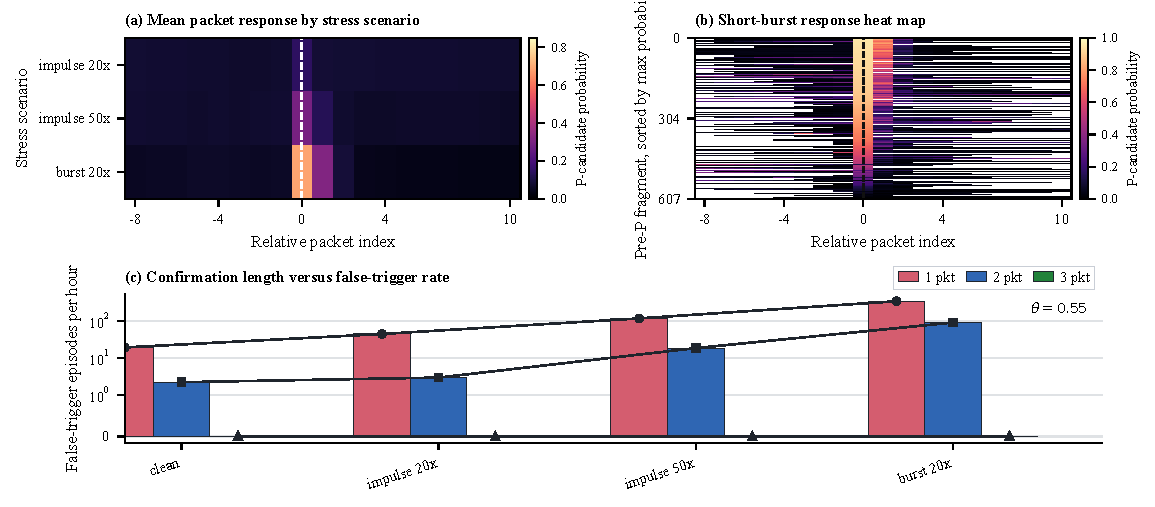
\includegraphics[width=\textwidth]{fig_spike_response_map_en}
  \caption{Spike-injected pre-P replay visualization. (a) Mean packet-level P-candidate response around injected transients for each stress scenario. (b) Segment-level heat map for the short packet-burst case, sorted by each fragment's maximum probability. (c) False-trigger episodes per hour under one-, two-, and three-packet confirmation. This controlled stress replay is separated from the station-time false-alarm rates in Table~\ref{tab:continuous_false_alarm}.}
  \label{fig:spike-response}
\end{figure*}

The spike, labeled-noise, and FDSN results identify the engineering failure mode: a strong short transient can mimic abrupt packet-to-packet feature change and rapid energy growth. Global threshold tightening or three-packet confirmation reduces this mode at a direct detection cost shown in Table~\ref{tab:falsealarm}. A narrow peak-width gate reduces the 50$\times$ impulse case from 18.79 to 1.50 two-packet episodes per hour with a conservative K-NET event-detection estimate of 97.8\%; a broader gate suppresses the packet-burst case to 1.50 episodes per hour and lowers that estimate to 84.5\%. A deployable chain should gate isolated peak-to-RMS outliers, one-sample spikes, clipping, component incoherence, and implausible artifact durations before model inference, then use multi-station coincidence and source-consistency checks after station-side confirmation. The final false-alert metric should be measured on broader chronological event-free streams as false alerts per station-day or network-day.

\subsection{Event-Window Multi-Station Association}
Table~\ref{tab:association} reports an event-window association simulation using the same K-NET station triggers. For each event, station trigger times are taken from the confirmation-completion packet, and an event is associated once at least $N$ distinct stations trigger within a rolling $W$-s window. The delay is measured from the earliest labeled P-arrival packet among the evaluated stations to the association time. This experiment tests whether independently generated station candidates retain event-level timing coherence after the single-station trigger stage. Station trigger times remain fixed during the association check.

\begin{table}[!t]
\centering
\caption{K-NET event-window multi-station association simulation at $\theta=0.55$ with two-packet single-station confirmation. Eligible events have at least the required number of stations. Delay is measured from the earliest labeled P-arrival packet among evaluated stations.}
\label{tab:association}
{\scriptsize\setlength{\tabcolsep}{1.45pt}\renewcommand{\arraystretch}{1.03}
\begin{tabular}{@{}lcccccccc@{}}
\toprule
Subset & Rule & Ev. & Elig. & Assoc. & All & Elig. & Med. & P95\\
\midrule
$M\geq4$ & 2 sta./3 s & 36 & 36 & 36 & 100.0\% & 100.0\% & 1.0 s & 3.75 s\\
$M\geq4$ & 3 sta./3 s & 36 & 36 & 36 & 100.0\% & 100.0\% & 2.0 s & 7.38 s\\
$M<4$ & 2 sta./3 s & 40 & 39 & 38 & 95.0\% & 97.4\% & 1.5 s & 5.80 s\\
$M<4$ & 3 sta./3 s & 40 & 36 & 34 & 85.0\% & 94.4\% & 2.0 s & 6.88 s\\
$M<4$ & 3 sta./5 s & 40 & 36 & 36 & 90.0\% & 100.0\% & 2.25 s & 8.13 s\\
\bottomrule
\end{tabular}}
\end{table}

For the $M\geq4$ K-NET subset, the three-station/3 s rule associates all 36 test events with a 2.0 s median delay and a 7.38 s P95 delay. For $M<4$, the three-station/3 s rule associates 34 of 40 events and 94.4\% of eligible events; expanding the window to 5 s associates all eligible small-event cases. These results support station-level trigger consistency under simple coincidence rules. Blind network association, hypocenter estimation, and magnitude estimation remain downstream tasks.

\FloatBarrier
\subsection{External Labeled and Continuous Evidence}
% Honest external-evidence closure for TGRS revision, 2026-06-17.
% Use as a replacement/addition to the external validation subsection.

\paragraph{External labeled accelerometer benchmark}
We evaluated the trained model on PNWAccelerometers, an independent public accelerometer dataset with labeled P-arrival annotations. The benchmark targets the model response around the labeled P arrival. A response near labeled P arrivals is counted by searching from three chunks before the labeled P-arrival chunk. This metric measures labeled onset sensitivity; full-stream first-trigger behavior is reported in the continuous replay check. Low-SNR accelerometer records reduce observable onset evidence, so we report a quality-stratified analysis and retain the unfiltered result as the low-SNR reference. On 1136 records with minimum component SNR at least 20 dB, the model reached an 84.2\% usable response near labeled P arrivals rate and an 83.7\% perfect response rate at $\theta=0.55$ with two consecutive positive chunks. The median timing gap was one chunk. A separate 500-record threshold-sensitivity audit kept the usable rate between 82.2\% and 88.0\% for $\theta$ from 0.45 to 0.60.

\paragraph{Continuous-stream false-trigger check}
We evaluated continuous behavior separately with CI strong-motion FDSN station-day replays. The check used 10 CI stations, four event-free six-hour windows plus seven event-free one-hour windows, and 308.05 station-hours of HN* strong-motion streams. At $\theta=0.55$ with two consecutive positive chunks, single-station outputs produced 107 trigger episodes over 12.84 station-days. A three-station short-window false-trigger check within 3--5 s produced zero three-station false-trigger clusters over the same event-free windows. The deployment interpretation is a station-side probability stream followed by network-level event confirmation.

\begin{table}[H]
\centering
\caption{External evidence closure. PNWAccelerometers evaluates labeled response near labeled P arrivals on public accelerometer records. CI/FDSN replays evaluate continuous false-trigger behavior on event-free strong-motion streams.}
\label{tab:external_evidence_closure}
{\tgrsdensetablesetup
\begin{tabular}{@{}p{0.29\columnwidth}p{0.64\columnwidth}@{}}
\toprule
Check & Evidence and interpretation \\
\midrule
External P labels & PNWAccelerometers SNR$\ge$20 dB, n=1136: 84.2\% usable, 83.7\% perfect; stable labeled response near labeled P arrivals. \\
Threshold sensitivity & PNWAccelerometers 500-record audit, $\theta=0.45$--0.60: 82.2--88.0\% usable; no narrow-threshold effect. \\
Low-SNR reference & PNWAccelerometers unfiltered random n=2000: 36.8\% usable; weak/low-SNR records remain difficult. \\
Single-station stream & CI/FDSN 12.84 station-days: 107 episodes; single-station alarms need confirmation. \\
Network stream & CI/FDSN three-station short-window false-trigger clusters in 3--5 s windows: 0 within event-free windows. \\
\bottomrule
\end{tabular}}
\end{table}

\paragraph{Scope of the evidence}
These experiments support a station-side probability stream with network-level event confirmation. The PNWAccelerometers result measures sensitivity near labeled P arrivals on labeled high-SNR accelerometer records. The CI/FDSN replay measures false-trigger behavior in continuous event-free streams. The unfiltered PNWAccelerometers subset reached a 36.8\% usable rate, identifying weak and low-SNR accelerometer records as the next quality tier.

\FloatBarrier

\subsection{Additional Diagnostics and Ablation}
Two supplementary diagnostics bound interpretation. A 500-trace synthetic noise stress test shows that both \modelv{} and PhaseNet degrade as SNR decreases. A lightweight intra-packet STA/LTA refiner reduces detected-trace MAE from 0.816 s to 0.383 s on an InstanceGM subset, showing that packet-level triggering can be paired with local sub-packet timing refinement. The held-out K-NET accelerometer set remains the main strong-motion validation.

Table~\ref{tab:ablation} evaluates the contribution of each model component by removing or modifying one design element at a time. Removing the delta feature causes the largest performance drop on InstanceGM, reducing the detection rate from 85.1\% to 4.9\%. This drop identifies inter-packet change as a central cue for causal onset recognition. Removing cumulative RMS normalization also reduces in-domain detection, showing that the normalization rule is part of the detector behavior. The 1.0 s packet variant increases the detection rate and coarsens the minimum decision interval, which is less suitable for near-source EEW.

\begin{table}[H]
\centering
\caption{Component ablation results under the ablation-run configuration. Metrics are computed on the same InstanceGM ablation subset; Aux. columns report the auxiliary-head diagnostic used in component analysis.}
\label{tab:ablation}
{\tgrsdensetablesetup
\begin{tabular}{@{}lccccc@{}}
\toprule
Variant & IG Det. & $\Delta$IG & Aux. Det. & $\Delta$Aux & Aux. Prec.\\
\midrule
Full model & 85.1 & -- & 87.4 & -- & 64.9\\
w/o pre-P aux. loss & 82.4 & -2.7 & 87.4 & 0.0 & 64.9\\
w/o delta feature & 4.9 & -80.2 & 48.8 & -38.5 & 20.5\\
w/o polarization & 82.5 & -2.6 & 61.5 & -25.9 & 85.7\\
w/o cumulative RMS & 69.6 & -15.5 & 92.7 & +5.3 & 9.8\\
w/o position enc. & 69.7 & -15.4 & 81.6 & -5.8 & 0.1\\
1.0 s packet & 86.7 & +1.7 & 93.0 & +5.6 & 43.1\\
\bottomrule
\end{tabular}}
\end{table}

\section{Discussion}
The central evidence is candidate availability on the station data stream. \modelv{} converts chronological accelerometer packets into a probability trace at packet close, so the First-P metric measures when a downstream module could first receive a P candidate. RED-PAN is the most relevant real-time neural comparator in this study and reaches a nearly identical usable rate on the common K-NET subset. \modelv{} reaches that operating range with a shorter packet-state update path and no missed records in the filtered K-NET test set. PhaseNet and EQTransformer are informative in a different way: their public fixed-window interfaces show how full-window organization, blinding, thresholds, and search regions shift first-trigger behavior under causal replay. Together these comparisons support a low-latency front-end design claim within the stated input-output setting.

The model's useful behavior comes from the combination of three simple physical cues. Cumulative RMS references the current packet to its own past background and keeps onset energy visible. The Z/NE channel supplies a compact particle-motion cue. Delta features expose the short-term change in learned waveform shape and energy. The ablation result supports this interpretation: removing delta features collapses InstanceGM detection, removing cumulative RMS causes a large decline, and removing Z/NE produces a smaller but measurable drop.

The data roles also shape the interpretation. InstanceGM contains both seismic-velocity and strong-motion acceleration records, so this article uses it as a broad representation-learning source. The strong-motion claim rests on independent K-NET accelerometer evaluation. Pilot instrument-family diagnostics remain supplementary evidence for data-domain limits; separating sensor-family behavior requires a larger verified acceleration benchmark.

The K-NET distance bins connect the method to near- and intermediate-field use. The 0--50 km group tests the tightest time budget, and the 100--200 km group tests weaker or more path-affected onsets. Similar usable rates across these bins show that the reported checkpoint preserved intermediate-distance stability within the filtered K-NET test set. The Iquique result remains lower and more early-biased, which points to the need for local calibration before applying the checkpoint to a new region.

The external evidence covers labeled response and continuous false-trigger behavior. PNWAccelerometers gives 85.0\% usable response on high-SNR labeled accelerometer records and 30.4\% on an unfiltered low-SNR reference subset. CI/FDSN supplies event-free continuous-stream exposure. Cross-network acceleration validation can extend to CESMD, ESM, CWA/TSMIP, and AFAD after their P-reference provenance is documented. Future validation should separate earliest weak-P evidence, which controls warning time, from later strong-energy growth, which is closer to engineering ground-motion products.

The practical output is a station candidate; alerting is a downstream network decision. Two-packet confirmation reduces clean K-NET pre-P false triggers to 2.25 episodes per hour and preserves 99.3\% K-NET event detection. The spike, STEAD, and CI/FDSN audits show why that candidate stream still needs artifact-aware station quality control and network logic. Event-window association shows that the same triggers can form simple multi-station coincidences in catalog-grouped K-NET events. The next system tier is chronological station-day evaluation with blind network association, source location, magnitude estimation, telemetry latency, and hardware-in-the-loop tests. P/S joint outputs, probability calibration, and quantized ARM or MCU runtime tests are natural engineering extensions.

\section{Conclusion}
This article presented \modelv, a strictly causal packet-level CNN--GRU picker for station-side P-wave candidate triggering in strong-motion acceleration streams. The model combines cumulative RMS normalization, a Z/NE particle-motion cue, causal convolution, delta features, and a unidirectional recurrent state, processing \chunk packets without future samples. It has 275,827 parameters, 0.32 ms mean single-thread CPU packet-step latency, 0.00 s median packet-index First-P delay, 98.3\% usable held-out K-NET strong-motion picks after multi-domain training, and 80.6\% usable Iquique blind-domain picks. On the common K-NET subset, it matches the usable performance of the official RED-PAN 60 s baseline with a shorter packet-state update path. External labeled-accelerometer and continuous-stream audits define the station quality-control, artifact-rejection, and network-association layer before alert issuance. These results support packet-level causal preprocessing and recurrent state updates as a practical front-end design for low-latency strong-motion P-candidate streams.

\section*{Code and Data Availability}
The supplementary release package provides the source code, model definition, evaluation commands, plotting scripts, environment specification, checkpoint manifest, split metadata, K-NET test identifiers, and confidence-interval tables. It records commands for all reported latency, replay, baseline, threshold, stratified, false-trigger, association, refinement, and ablation analyses. Public waveform data are obtained from their original providers: INSTANCE/InstanceGM through the INSTANCE release and SeisBench, the K-NET-derived Japan earthquake dataset through Mendeley Data \cite{sarkar2022japan}, SeisBench-hosted PNWAccelerometers and Iquique benchmark records through their original data sources \cite{woollam2019iquique,woollam2022seisbench}, CI continuous strong-motion waveforms through FDSN services, and original K-NET strong-motion records from NIED \cite{nied2019knet}. The supplementary package provides record identifiers and preprocessing scripts; raw third-party waveforms are not redistributed. A public repository or DOI archive can be frozen after final review for long-term access.

\section*{Acknowledgment}
This work received no specific grant from any funding agency in the public, commercial, or not-for-profit sectors.
The authors thank NIED for operating and maintaining K-NET, Sarkar et al. for releasing the annotated Japan earthquake dataset through Mendeley Data, and the SeisBench ecosystem for enabling reproducible benchmarking.
AI-based language tools were used only for grammar enhancement. The authors verified the manuscript and all scientific results; no AI tool generated experimental data, analyses, or scientific figures.

\bibliographystyle{IEEEtran}
\bibliography{references}

\end{document}
